\documentclass[12pt,letterpaper]{article}\usepackage[]{graphicx}\usepackage[]{color}
%% maxwidth is the original width if it is less than linewidth
%% otherwise use linewidth (to make sure the graphics do not exceed the margin)
\makeatletter
\def\maxwidth{ %
  \ifdim\Gin@nat@width>\linewidth
    \linewidth
  \else
    \Gin@nat@width
  \fi
}
\makeatother

\definecolor{fgcolor}{rgb}{0.345, 0.345, 0.345}
\newcommand{\hlnum}[1]{\textcolor[rgb]{0.686,0.059,0.569}{#1}}%
\newcommand{\hlstr}[1]{\textcolor[rgb]{0.192,0.494,0.8}{#1}}%
\newcommand{\hlcom}[1]{\textcolor[rgb]{0.678,0.584,0.686}{\textit{#1}}}%
\newcommand{\hlopt}[1]{\textcolor[rgb]{0,0,0}{#1}}%
\newcommand{\hlstd}[1]{\textcolor[rgb]{0.345,0.345,0.345}{#1}}%
\newcommand{\hlkwa}[1]{\textcolor[rgb]{0.161,0.373,0.58}{\textbf{#1}}}%
\newcommand{\hlkwb}[1]{\textcolor[rgb]{0.69,0.353,0.396}{#1}}%
\newcommand{\hlkwc}[1]{\textcolor[rgb]{0.333,0.667,0.333}{#1}}%
\newcommand{\hlkwd}[1]{\textcolor[rgb]{0.737,0.353,0.396}{\textbf{#1}}}%

\usepackage{framed}
\makeatletter
\newenvironment{kframe}{%
 \def\at@end@of@kframe{}%
 \ifinner\ifhmode%
  \def\at@end@of@kframe{\end{minipage}}%
  \begin{minipage}{\columnwidth}%
 \fi\fi%
 \def\FrameCommand##1{\hskip\@totalleftmargin \hskip-\fboxsep
 \colorbox{shadecolor}{##1}\hskip-\fboxsep
     % There is no \\@totalrightmargin, so:
     \hskip-\linewidth \hskip-\@totalleftmargin \hskip\columnwidth}%
 \MakeFramed {\advance\hsize-\width
   \@totalleftmargin\z@ \linewidth\hsize
   \@setminipage}}%
 {\par\unskip\endMakeFramed%
 \at@end@of@kframe}
\makeatother

\definecolor{shadecolor}{rgb}{.97, .97, .97}
\definecolor{messagecolor}{rgb}{0, 0, 0}
\definecolor{warningcolor}{rgb}{1, 0, 1}
\definecolor{errorcolor}{rgb}{1, 0, 0}
\newenvironment{knitrout}{}{} % an empty environment to be redefined in TeX

\usepackage{alltt}
 \usepackage[left=2cm,right=2cm,top=2cm,bottom=2cm]{geometry}
\usepackage[ansinew]{inputenc}
\usepackage[spanish]{babel}
\usepackage{amsmath}
\usepackage{amsfonts}
\usepackage{amssymb}
\usepackage{dsfont}
\usepackage{multicol} 
\usepackage{subfigure}
\usepackage{graphicx}
\usepackage{float} 
\usepackage{verbatim} 
\usepackage[left=2cm,right=2cm,top=2cm,bottom=2cm]{geometry}
\usepackage{fancyhdr}
\pagestyle{fancy} 
\fancyhead[LO]{\leftmark}
\usepackage{caption}
\newtheorem{definicion}{Definci\'on}
\IfFileExists{upquote.sty}{\usepackage{upquote}}{}
\begin{document}

\begin{titlepage}
\setlength{\unitlength}{1 cm} %Especificar unidad de trabajo


\begin{center}
\textbf{{\large UNIVERSIDAD DE EL SALVADOR}\\
{\large FACULTAD MULTIDISCIPLINARIA DE OCCIDENTE}\\
{\large DEPARTAMENTO DE MATEM\'ATICA}}\\[0.50 cm]

\begin{picture}(18,4)
 \put(7,0){
\includegraphics[width=4cm]{minerva.jpg}}
\end{picture}
\\[0.25 cm]

\textbf{{\large Licenciatura en Estad\'istica}\\[1.25cm]
{\large Control Estadistico del Paquete R }\\[2 cm]
%\setlength{\unitlength}{1 cm}
{\large  \textbf{''UNIDAD TRES"}}\\
{\large  \textbf{Pr\'actica 09-An\'alisis de una variable bidimensional categ\'orica.}}\\[3 cm]
{\large Alumna:}\\
{\large Martha Yoana Medina S\'anchez}\\[2cm]
{\large Fecha de elaboraci\'on}\\
Santa Ana - \today }
\end{center}
\end{titlepage}

\newtheorem{teorema}{Teorema}
\newtheorem{prop}{Proposici\'on}[section]

\lhead{UNIDAD TRES}
\chead{PR\'ACTICA 09}
\lfoot{LICENCIATURA EN ESTAD\'ISTICA}
\cfoot{UESOCC}
\rfoot{\thepage}
%\pagestyle{fancy} 

\setcounter{page}{1}
\newpage

\begin{center}
\textbf{Pr\'actica 09-An\'alisis de unavariable bidimensional categórica.}
\subsection*{REALICE UN AN\'ALISIS ESTAD\'ISTICO DE LOS DATOS.}
\end{center}

\begin{enumerate}
  \item Activa tu directorio de trabajo.
\begin{knitrout}
\definecolor{shadecolor}{rgb}{0.969, 0.969, 0.969}\color{fgcolor}\begin{kframe}
\begin{alltt}
\hlkwd{getwd}\hlstd{()}
\end{alltt}
\begin{verbatim}
## [1] "C:/Users/User/Documents/PRACTICAS_YOANA_MEDINA/Yoana/PRACTICAS DE R"
\end{verbatim}
\begin{alltt}
\hlkwd{setwd}\hlstd{(}\hlstr{"C:/Users/User/Documents/PRACTICAS_YOANA_MEDINA/Yoana/PRACTICAS DE R"}\hlstd{)}
\end{alltt}
\end{kframe}
\end{knitrout}

\item Limpia de objetos el \'area de trabajo (Workspace).
\begin{knitrout}
\definecolor{shadecolor}{rgb}{0.969, 0.969, 0.969}\color{fgcolor}\begin{kframe}
\begin{alltt}
\hlkwd{ls}\hlstd{()}
\end{alltt}
\begin{verbatim}
## character(0)
\end{verbatim}
\begin{alltt}
\hlkwd{rm}\hlstd{(}\hlkwc{list}\hlstd{=}\hlkwd{ls}\hlstd{(}\hlkwc{all}\hlstd{=}\hlnum{TRUE}\hlstd{))}
\hlkwd{ls}\hlstd{()}
\end{alltt}
\begin{verbatim}
## character(0)
\end{verbatim}
\end{kframe}
\end{knitrout}

\item Crea un nuevo Script y ll\'amale "Script09-DatosBivariados1".

\item Crea en Excel una hoja de datos con dos columnas o variables 
\begin{knitrout}
\definecolor{shadecolor}{rgb}{0.969, 0.969, 0.969}\color{fgcolor}\begin{kframe}
\begin{alltt}
\hlcom{# Recuerda que al guardar la hoja, el tipo de archivo es de extension .csv}
\hlcom{# (delimitado por comas). }
\hlcom{# Llamale al archivo: HojaCat }
\end{alltt}
\end{kframe}
\end{knitrout}
\begin{knitrout}
\definecolor{shadecolor}{rgb}{0.969, 0.969, 0.969}\color{fgcolor}\begin{kframe}
\begin{alltt}
\hlcom{# Otra forma de crear la hoja de datos es la siguiente (Vea la }
\hlcom{# Practica 04): Primero crear las dos variables categoricas en un }
\hlcom{# editor de texto como NotePad o WordPad, colocando nombre a cada }
\hlcom{# columna, y llamandole "HojaCat.txt". }
\end{alltt}
\end{kframe}
\end{knitrout}
\begin{knitrout}
\definecolor{shadecolor}{rgb}{0.969, 0.969, 0.969}\color{fgcolor}\begin{kframe}
\begin{alltt}
\hlcom{# Luego puede leer o recuperar este archivo con la funciOn read.table() }
\hlstd{HojaCat} \hlkwb{<-} \hlkwd{read.table}\hlstd{(}\hlstr{"HojaCat.txt"}\hlstd{,} \hlkwc{header}\hlstd{=}\hlnum{TRUE}\hlstd{)}
\hlstd{HojaCat}
\end{alltt}
\begin{verbatim}
## [1] VAR   X1    VAR.1 X2   
## <0 rows> (or 0-length row.names)
\end{verbatim}
\end{kframe}
\end{knitrout}

\item Recupera desde el entorno de R la hoja de datos de Excel.
\begin{knitrout}
\definecolor{shadecolor}{rgb}{0.969, 0.969, 0.969}\color{fgcolor}\begin{kframe}
\begin{alltt}
\hlstd{HojaCat} \hlkwb{<-} \hlkwd{read.csv}\hlstd{(}\hlstr{"HojaCat.csv"}\hlstd{,} \hlkwc{strip.white}\hlstd{=}\hlnum{TRUE}\hlstd{);HojaCat}
\end{alltt}
\begin{verbatim}
##    Estado.Civil  Ocupacion
## 1        casado desocupado
## 2       soltero    estudia
## 3       soltero    trabaja
## 4        casado    estudia
## 5    acompanado    trabaja
## 6       soltero desocupado
## 7        casado    trabaja
## 8        casado    estudia
## 9    acompanado desocupado
## 10   acompanado    estudia
## 11       casado    trabaja
## 12      soltero    estudia
## 13   acompanado desocupado
## 14       casado desocupado
## 15      soltero    estudia
## 16      soltero    trabaja
## 17       casado desocupado
## 18      soltero    trabaja
\end{verbatim}
\end{kframe}
\end{knitrout}

\item Conecta la hoja de datos a la segunda ruta o lista de b\'usqueda.
\begin{knitrout}
\definecolor{shadecolor}{rgb}{0.969, 0.969, 0.969}\color{fgcolor}\begin{kframe}
\begin{alltt}
\hlkwd{attach}\hlstd{(HojaCat,} \hlkwc{pos}\hlstd{=}\hlnum{2}\hlstd{)}

\hlcom{# pos especifica la posicion donde buscar la conexion }

\hlkwd{search}\hlstd{()}
\end{alltt}
\begin{verbatim}
##  [1] ".GlobalEnv"        "HojaCat"           "package:knitr"    
##  [4] "package:stats"     "package:graphics"  "package:grDevices"
##  [7] "package:utils"     "package:datasets"  "package:methods"  
## [10] "Autoloads"         "package:base"
\end{verbatim}
\end{kframe}
\end{knitrout}

\item Crea una tabla de contigencia o de doble entrada
\begin{knitrout}
\definecolor{shadecolor}{rgb}{0.969, 0.969, 0.969}\color{fgcolor}\begin{kframe}
\begin{alltt}
\hlstd{tablaCont} \hlkwb{<-} \hlkwd{table}\hlstd{(HojaCat); tablaCont}
\end{alltt}
\begin{verbatim}
##             Ocupacion
## Estado.Civil desocupado estudia trabaja
##   acompanado          2       1       1
##   casado              3       2       2
##   soltero             1       3       3
\end{verbatim}
\begin{alltt}
\hlkwd{length}\hlstd{(HojaCat)}
\end{alltt}
\begin{verbatim}
## [1] 2
\end{verbatim}
\begin{alltt}
\hlcom{# Note que esta instruccion no devuelve el numero de elementos, sino mas}
\hlcom{# bien el numero de variables o columnas consideradas en el conjunto de}
\hlcom{# datos. }
\end{alltt}
\end{kframe}
\end{knitrout}

\begin{knitrout}
\definecolor{shadecolor}{rgb}{0.969, 0.969, 0.969}\color{fgcolor}\begin{kframe}
\begin{alltt}
\hlcom{# Encuentra la suma de cada fila de la tabla de contingencia }

\hlcom{# Distribucion marginal de }
\hlstd{X}\hlkwb{=}\hlstr{"Estado civil"}

\hlstd{suma.filas} \hlkwb{<-} \hlkwd{apply}\hlstd{(tablaCont,} \hlnum{1}\hlstd{, sum); suma.filas}
\end{alltt}
\begin{verbatim}
## acompanado     casado    soltero 
##          4          7          7
\end{verbatim}
\begin{alltt}
\hlcom{# El 1 indica que son totales por fila }
\end{alltt}
\end{kframe}
\end{knitrout}

\begin{knitrout}
\definecolor{shadecolor}{rgb}{0.969, 0.969, 0.969}\color{fgcolor}\begin{kframe}
\begin{alltt}
\hlcom{# Encuentra la suma de cada filade la tabla de contingencia }
\hlcom{# distribución marginal de }
\hlstd{Y}\hlkwb{=}\hlstr{"Ocupaci\textbackslash{}'on"}
\hlstd{suma.columnas} \hlkwb{<-} \hlkwd{apply}\hlstd{(tablaCont,}\hlnum{2}\hlstd{,sum); suma.columnas}
\end{alltt}
\begin{verbatim}
## desocupado    estudia    trabaja 
##          6          6          6
\end{verbatim}
\begin{alltt}
\hlcom{# 2 indica que son totales por columna }
\end{alltt}
\end{kframe}
\end{knitrout}

 
\begin{knitrout}
\definecolor{shadecolor}{rgb}{0.969, 0.969, 0.969}\color{fgcolor}\begin{kframe}
\begin{alltt}
\hlcom{# Graficos de barras para tabla de contingencia.}

\hlcom{# Barras apiladas }

\hlkwd{barplot}\hlstd{(}\hlkwd{t}\hlstd{(tablaCont),} \hlkwc{main}\hlstd{=}\hlstr{"Gr\textbackslash{}'afico de barras (Estado Civil, 
        Ocupación)"}\hlstd{,} \hlkwc{xlab}\hlstd{=}\hlstr{"Estado civil"}\hlstd{,} \hlkwc{ylab}\hlstd{=}\hlstr{"Ocupaci\textbackslash{}'on"}\hlstd{,}
        \hlkwc{col}\hlstd{=}\hlkwd{c}\hlstd{(}\hlstr{"red"}\hlstd{,} \hlstr{"blue"}\hlstd{,} \hlstr{"orange"}\hlstd{),} \hlkwc{legend.text}\hlstd{=}\hlnum{TRUE}\hlstd{)}
\end{alltt}
\end{kframe}
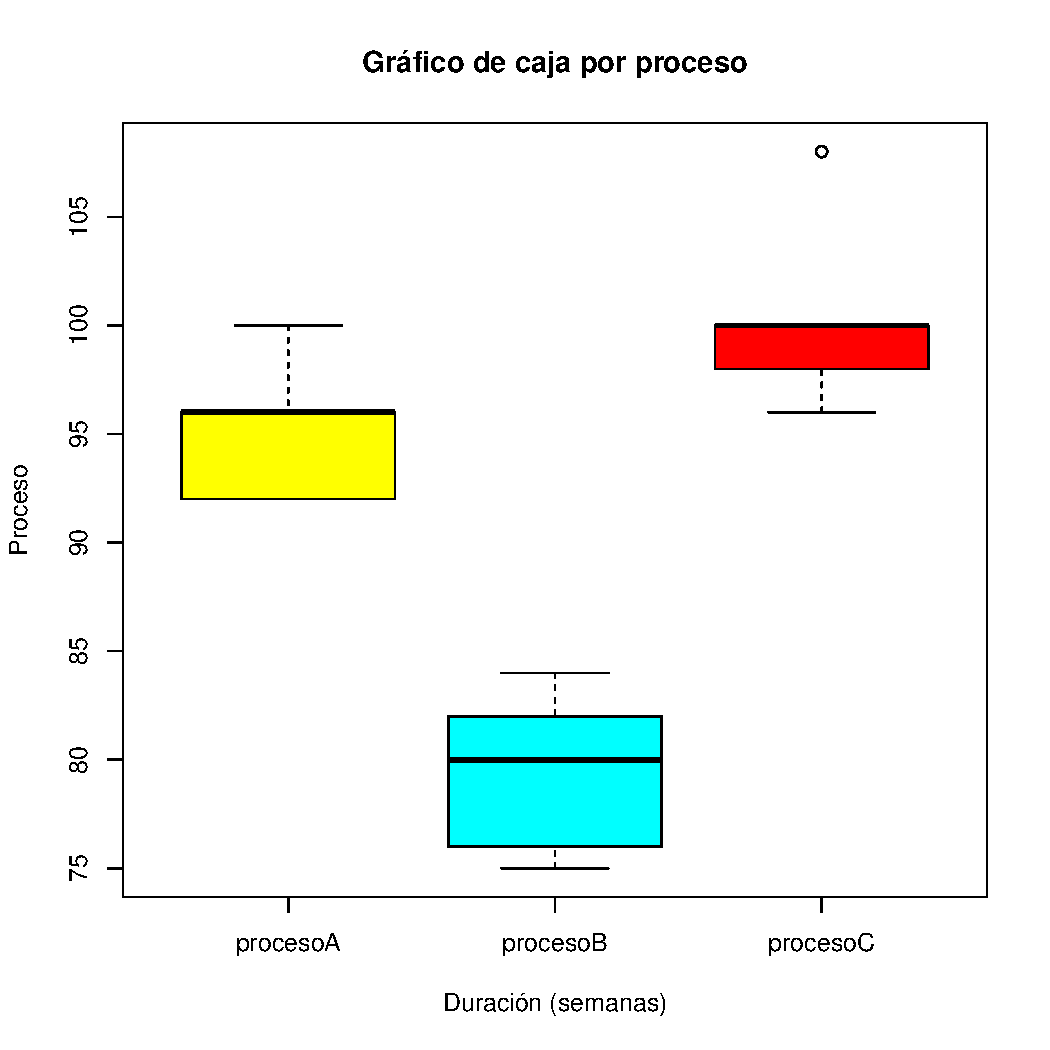
\includegraphics[width=\maxwidth]{figure/unnamed-chunk-11-1} 
\begin{kframe}\begin{alltt}
\hlcom{# Note que t(tablaCont) indica que las barras representan el Estado civil}
\hlcom{# de los encuestados y que estas se subdividen en cada una de las }
\hlcom{# diferentes ocupaciones consideradas.}

\hlcom{# En caso de usar unicamente tablaCont; las barras representaran las}
\hlcom{# diferentes ocupaciones y estas estaran subdividas en cada uno de los}
\hlcom{# estados civiles. }
\end{alltt}
\end{kframe}
\end{knitrout}

\begin{knitrout}
\definecolor{shadecolor}{rgb}{0.969, 0.969, 0.969}\color{fgcolor}\begin{kframe}
\begin{alltt}
\hlcom{# Barras agrupadas}

\hlkwd{barplot}\hlstd{(}\hlkwd{t}\hlstd{(tablaCont),} \hlkwc{main}\hlstd{=}\hlstr{"Gráfico de barras (Estado, Ocupación)"}\hlstd{,}
        \hlkwc{xlab}\hlstd{=}\hlstr{"Estado civil"}\hlstd{,} \hlkwc{ylab}\hlstd{=}\hlstr{"Ocupación"}\hlstd{,} \hlkwc{beside}\hlstd{=}\hlnum{TRUE}\hlstd{,}
        \hlkwc{col}\hlstd{=}\hlkwd{c}\hlstd{(}\hlstr{"red"}\hlstd{,} \hlstr{"blue"}\hlstd{,} \hlstr{"orange"}\hlstd{),}\hlkwc{legend.text}\hlstd{=}\hlnum{TRUE}\hlstd{)}
\end{alltt}
\end{kframe}
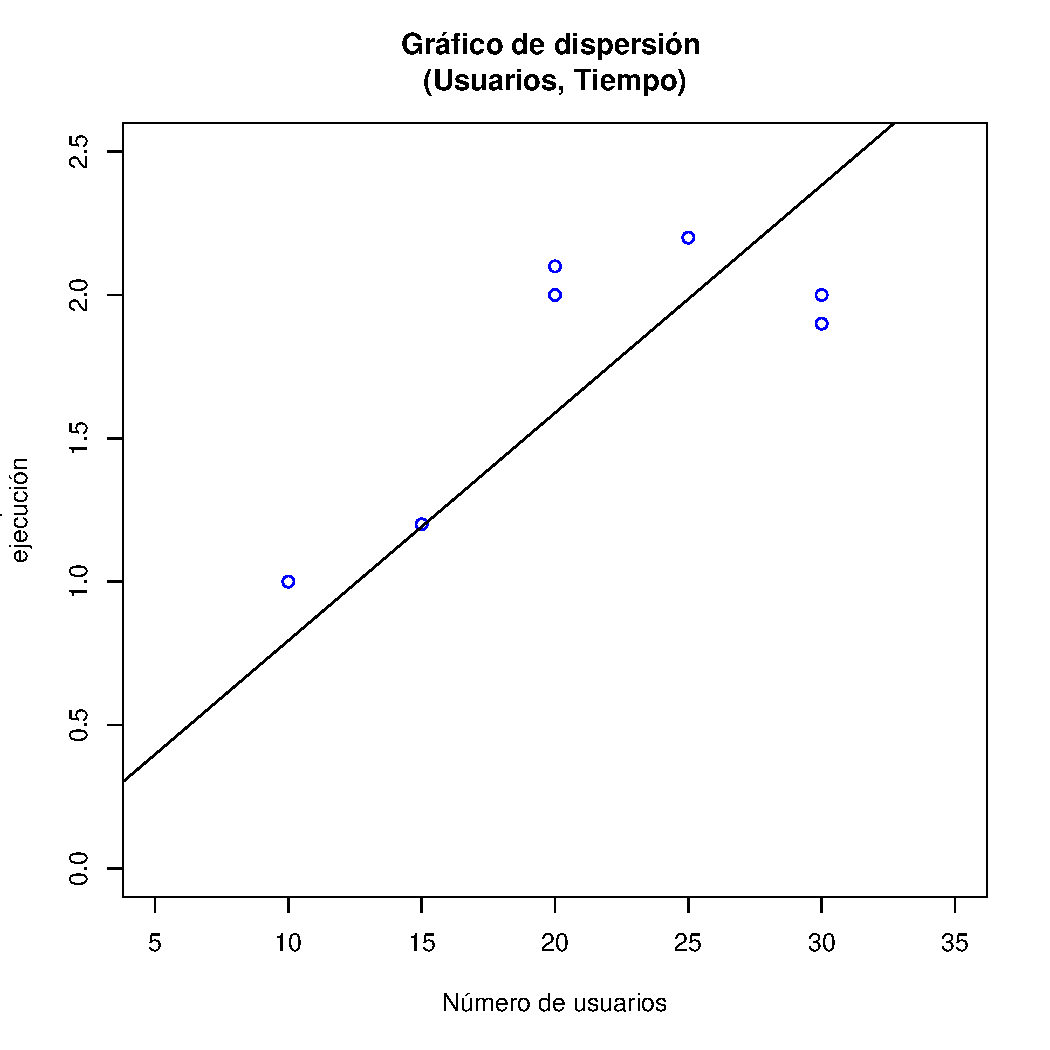
\includegraphics[width=\maxwidth]{figure/unnamed-chunk-12-1} 
\begin{kframe}\begin{alltt}
\hlcom{# Note que la instruccion beside =TRUE, indica que por cada una de las}
\hlcom{# diferentes ocupaciones se creara una barra para cada estado civil. Note}
\hlcom{# que al usar beside =FALSE se obtiene el mismo grafico de la instruccion}
\hlcom{# anterior. }
\end{alltt}
\end{kframe}
\end{knitrout}

\begin{knitrout}
\definecolor{shadecolor}{rgb}{0.969, 0.969, 0.969}\color{fgcolor}\begin{kframe}
\begin{alltt}
\hlkwd{barplot}\hlstd{(tablaCont,} \hlkwc{main}\hlstd{=}\hlstr{"Gráfico de barras (Ocupación, Estado)"}\hlstd{,}
        \hlkwc{xlab}\hlstd{=}\hlstr{"Ocupación\textbackslash{}n"}\hlstd{,} \hlkwc{ylab}\hlstd{=}\hlstr{"Estado civil"}\hlstd{,} \hlkwc{beside}\hlstd{=}\hlnum{TRUE}\hlstd{,}
        \hlkwc{col}\hlstd{=}\hlkwd{c}\hlstd{(}\hlstr{"red"}\hlstd{,} \hlstr{"blue"}\hlstd{,} \hlstr{"orange"}\hlstd{),}\hlkwc{legend.text}\hlstd{=}\hlnum{TRUE}\hlstd{)}
\end{alltt}
\end{kframe}
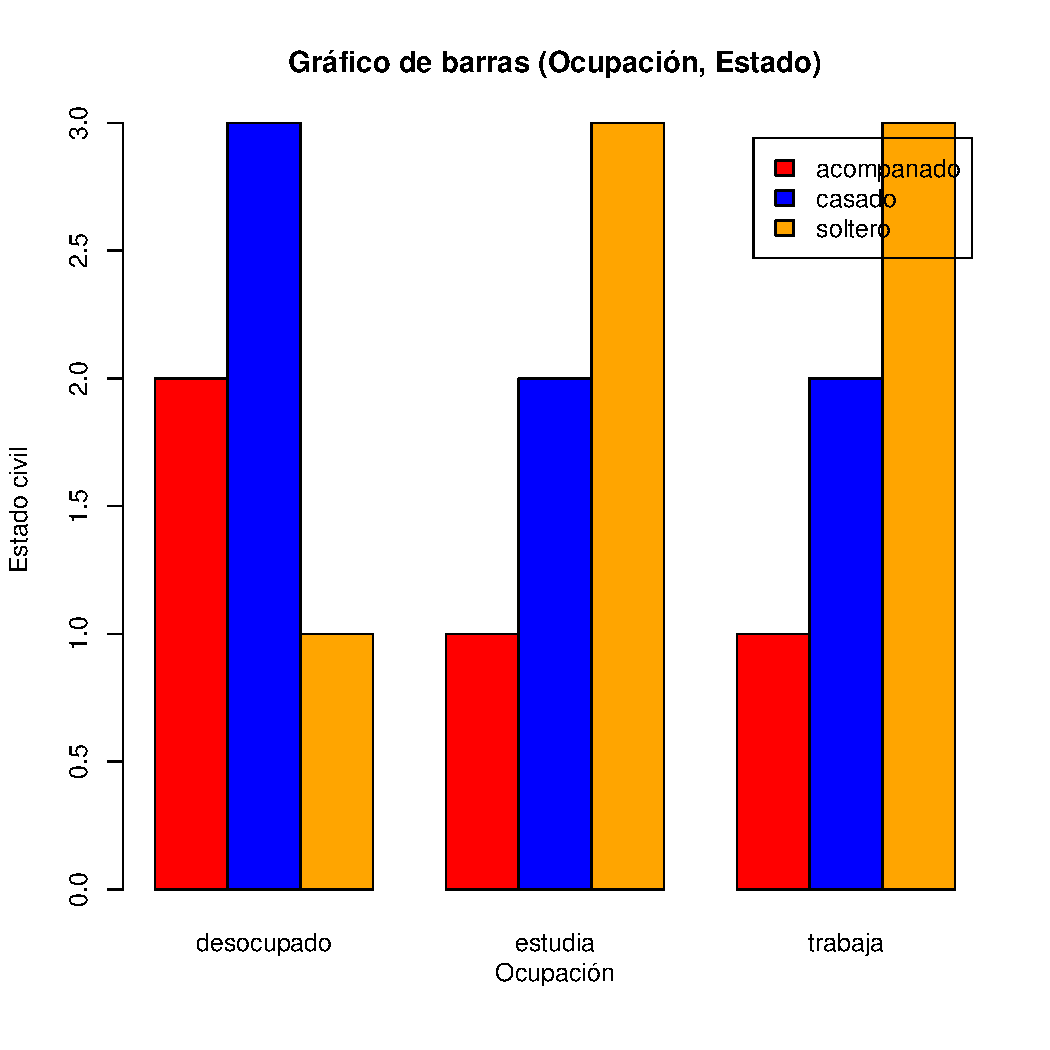
\includegraphics[width=\maxwidth]{figure/unnamed-chunk-13-1} 

\end{knitrout}

\item Calcula tablas de proporciones o de probabilidades. 
\begin{knitrout}
\definecolor{shadecolor}{rgb}{0.969, 0.969, 0.969}\color{fgcolor}\begin{kframe}
\begin{alltt}
\hlcom{# Guardar las todas las opciones iniciales y modificar numero }
\hlcom{# de decimales }

\hlstd{op} \hlkwb{<-} \hlkwd{options}\hlstd{()}
\hlkwd{options}\hlstd{(}\hlkwc{digits}\hlstd{=}\hlnum{3}\hlstd{)} \hlcom{# sólo imprime 3 lugares decimales }
\hlkwd{options}\hlstd{(}\hlstr{'digits'}\hlstd{)}
\end{alltt}
\begin{verbatim}
## $digits
## [1] 3
\end{verbatim}
\end{kframe}
\end{knitrout}

\begin{knitrout}
\definecolor{shadecolor}{rgb}{0.969, 0.969, 0.969}\color{fgcolor}\begin{kframe}
\begin{alltt}
\hlcom{# Proporciones basadas en el total de la muestra, la suma de filas y}
\hlcom{# columnas suman 1.}

\hlstd{propTotal} \hlkwb{<-} \hlkwd{prop.table}\hlstd{(tablaCont); propTotal}
\end{alltt}
\begin{verbatim}
##             Ocupacion
## Estado.Civil desocupado estudia trabaja
##   acompanado     0.1111  0.0556  0.0556
##   casado         0.1667  0.1111  0.1111
##   soltero        0.0556  0.1667  0.1667
\end{verbatim}
\begin{alltt}
\hlkwd{barplot}\hlstd{(}\hlkwd{t}\hlstd{(propTotal),} \hlkwc{main}\hlstd{=}\hlstr{"Gráfico de barras (Estado, Ocupación)"}\hlstd{,}
        \hlkwc{xlab}\hlstd{=}\hlstr{"Estado civil\textbackslash{}n"}\hlstd{,} \hlkwc{ylab}\hlstd{=}\hlstr{"Ocupación"}\hlstd{,} \hlkwc{beside}\hlstd{=}\hlnum{TRUE}\hlstd{,}
        \hlkwc{col}\hlstd{=}\hlkwd{c}\hlstd{(}\hlstr{"red"}\hlstd{,} \hlstr{"blue"}\hlstd{,} \hlstr{"orange"}\hlstd{),}\hlkwc{legend.text}\hlstd{=}\hlnum{TRUE}\hlstd{)}
\end{alltt}
\end{kframe}
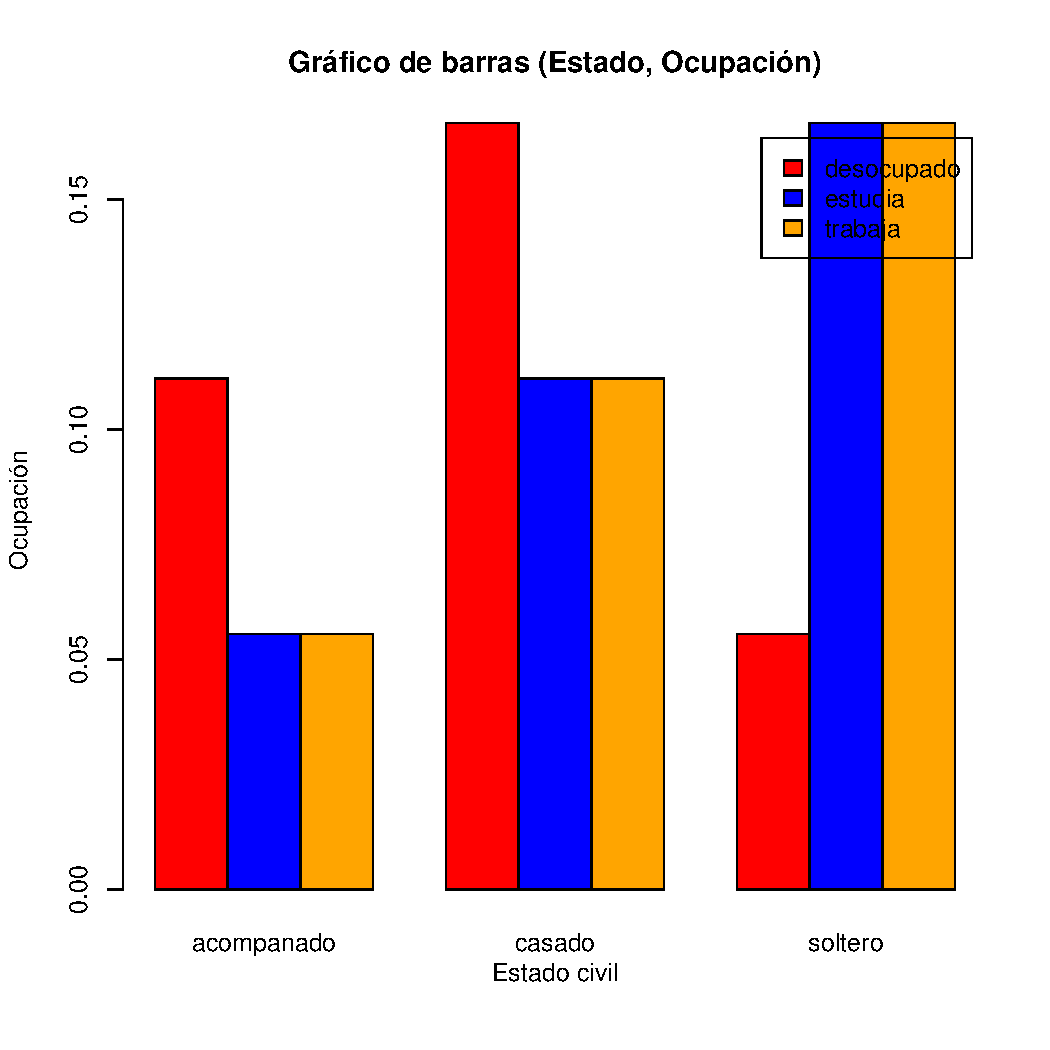
\includegraphics[width=\maxwidth]{figure/unnamed-chunk-15-1} 

\end{knitrout}

\begin{knitrout}
\definecolor{shadecolor}{rgb}{0.969, 0.969, 0.969}\color{fgcolor}\begin{kframe}
\begin{alltt}
\hlcom{# Proporciones basadas en el total por fila, cada fila suma 1.}

\hlstd{propFila} \hlkwb{<-} \hlkwd{prop.table}\hlstd{(tablaCont,} \hlnum{1}\hlstd{); propFila}
\end{alltt}
\begin{verbatim}
##             Ocupacion
## Estado.Civil desocupado estudia trabaja
##   acompanado      0.500   0.250   0.250
##   casado          0.429   0.286   0.286
##   soltero         0.143   0.429   0.429
\end{verbatim}
\begin{alltt}
\hlcom{# Total por fila se indica en 1 }

\hlkwd{barplot}\hlstd{(}\hlkwd{t}\hlstd{(propFila),} \hlkwc{main}\hlstd{=}\hlstr{"Gráfico de barras (Estado, Ocupación)"}\hlstd{,}
        \hlkwc{xlab}\hlstd{=}\hlstr{"Estado civil\textbackslash{}n"}\hlstd{,} \hlkwc{ylab}\hlstd{=}\hlstr{"Ocupación"}\hlstd{,} \hlkwc{beside}\hlstd{=}\hlnum{TRUE}\hlstd{,}
        \hlkwc{col}\hlstd{=}\hlkwd{c}\hlstd{(}\hlstr{"red"}\hlstd{,} \hlstr{"blue"}\hlstd{,} \hlstr{"orange"}\hlstd{),} \hlkwc{legend.text}\hlstd{=}\hlnum{TRUE}\hlstd{)}
\end{alltt}
\end{kframe}
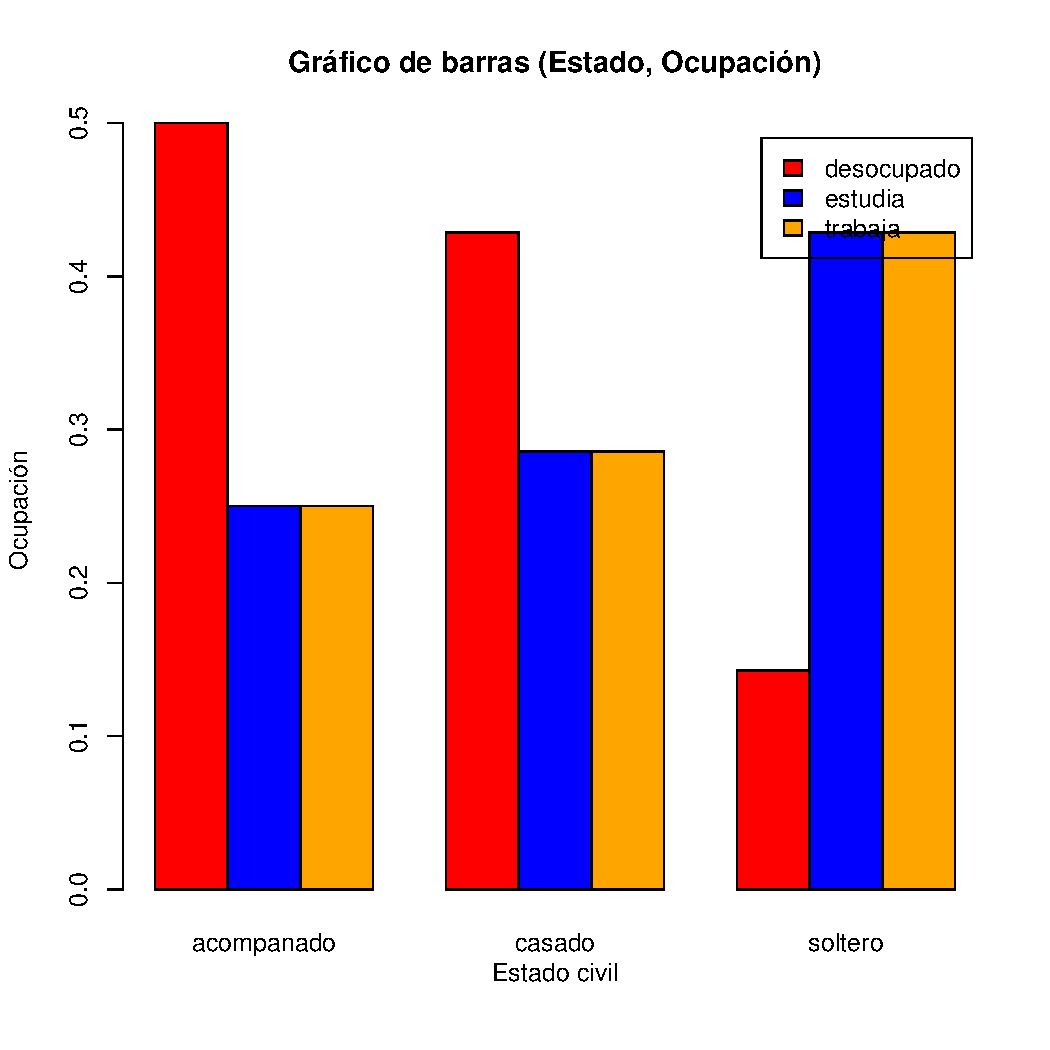
\includegraphics[width=\maxwidth]{figure/unnamed-chunk-16-1} 

\end{knitrout}

\begin{knitrout}
\definecolor{shadecolor}{rgb}{0.969, 0.969, 0.969}\color{fgcolor}\begin{kframe}
\begin{alltt}
\hlcom{# Proporciones basadas en el total por columna, cada columna suma 1.}

\hlstd{propColum} \hlkwb{<-} \hlkwd{prop.table}\hlstd{(tablaCont,} \hlnum{2}\hlstd{); propColum}
\end{alltt}
\begin{verbatim}
##             Ocupacion
## Estado.Civil desocupado estudia trabaja
##   acompanado      0.333   0.167   0.167
##   casado          0.500   0.333   0.333
##   soltero         0.167   0.500   0.500
\end{verbatim}
\begin{alltt}
\hlcom{# Total por columna se indica en 2 }

\hlkwd{barplot}\hlstd{(propColum,} \hlkwc{main}\hlstd{=}\hlstr{"Gráfico de barras (Ocupación, Estado)"}\hlstd{,}
        \hlkwc{xlab}\hlstd{=}\hlstr{"Ocupación\textbackslash{}n"}\hlstd{,} \hlkwc{ylab}\hlstd{=}\hlstr{"Estado civil"}\hlstd{,} \hlkwc{beside}\hlstd{=}\hlnum{TRUE}\hlstd{,}
        \hlkwc{col}\hlstd{=}\hlkwd{c}\hlstd{(}\hlstr{"red"}\hlstd{,} \hlstr{"blue"}\hlstd{,} \hlstr{"orange"}\hlstd{),}\hlkwc{legend.text}\hlstd{=}\hlnum{TRUE}\hlstd{)}
\end{alltt}
\end{kframe}
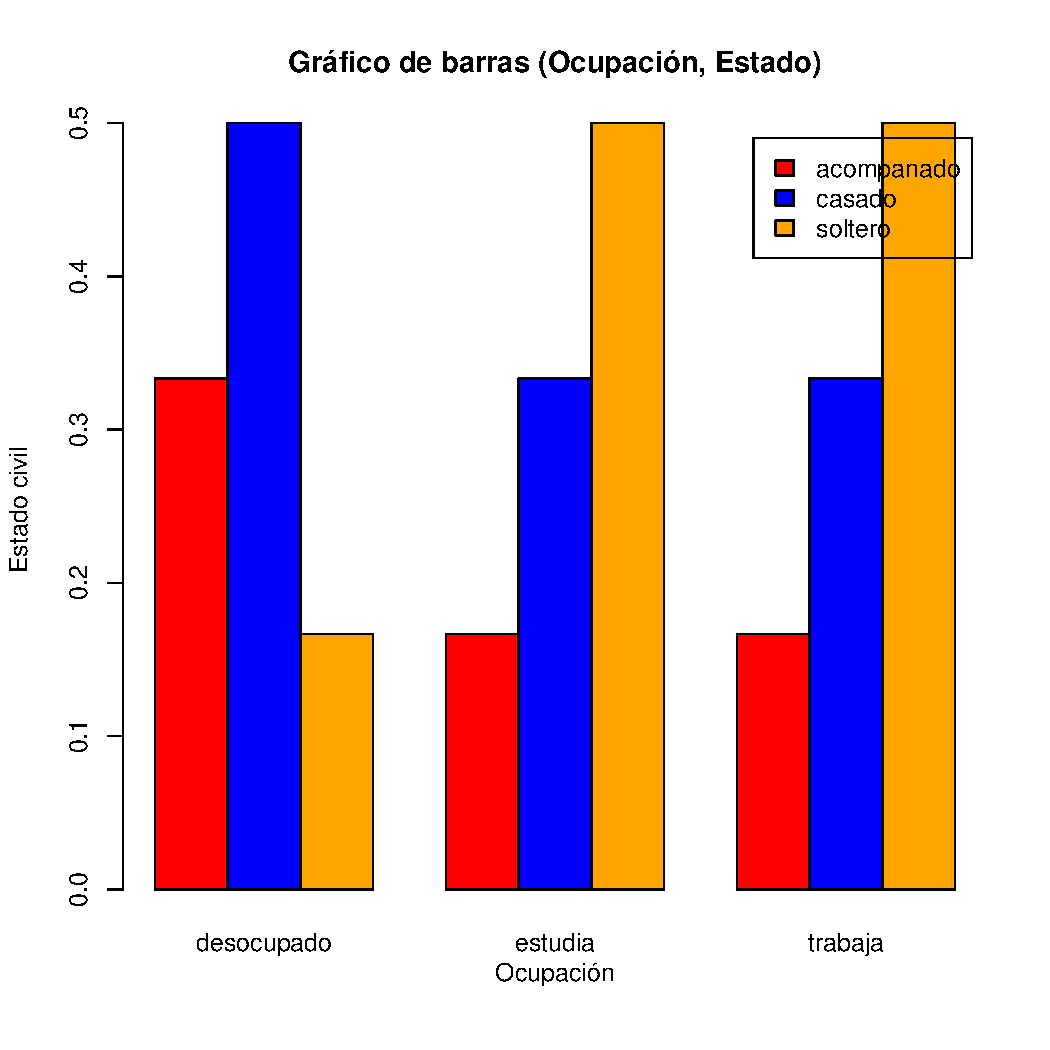
\includegraphics[width=\maxwidth]{figure/unnamed-chunk-17-1} 

\end{knitrout}

\item Otra forma de elaborar los gr\'aficos de barras para el vector bidimensional categ\'orico. 

\begin{knitrout}
\definecolor{shadecolor}{rgb}{0.969, 0.969, 0.969}\color{fgcolor}\begin{kframe}
\begin{alltt}
\hlcom{# Gráfico de barras no apiladas y colocación de leyenda}

\hlkwd{barplot}\hlstd{(}\hlkwd{table}\hlstd{(HojaCat),} \hlkwc{main}\hlstd{=}\hlstr{"Gráfico de barras (Estado, Ocupación)"}\hlstd{,}
        \hlkwc{xlab} \hlstd{=} \hlstr{"Estado civil"}\hlstd{,}  \hlkwc{ylab}\hlstd{=}\hlstr{"Ocupación"}\hlstd{,} \hlkwc{beside}\hlstd{=}\hlnum{TRUE}\hlstd{,}
        \hlkwc{col}\hlstd{=}\hlkwd{c}\hlstd{(}\hlstr{"red"}\hlstd{,} \hlstr{"blue"}\hlstd{,} \hlstr{"orange"}\hlstd{),} \hlkwc{legend.text}\hlstd{=T)}
\end{alltt}
\end{kframe}
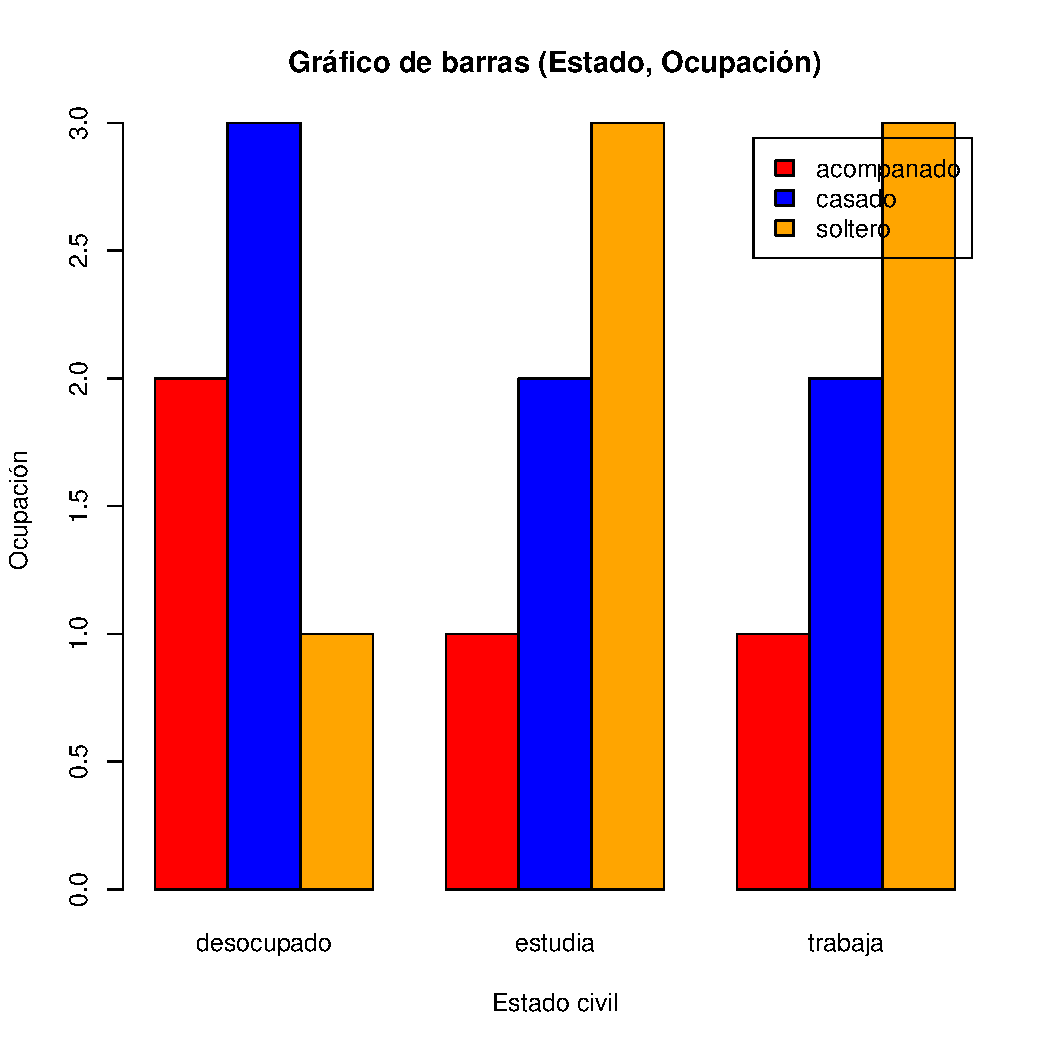
\includegraphics[width=\maxwidth]{figure/unnamed-chunk-18-1} 

\end{knitrout}

\begin{knitrout}
\definecolor{shadecolor}{rgb}{0.969, 0.969, 0.969}\color{fgcolor}\begin{kframe}
\begin{alltt}
\hlkwd{barplot}\hlstd{(}\hlkwd{table}\hlstd{(HojaCat),} \hlkwc{main}\hlstd{=}\hlstr{"Gráfico de barras (Ocupación, Estado)"}\hlstd{,}
        \hlkwc{xlab} \hlstd{=} \hlstr{"Ocupación"}\hlstd{,} \hlkwc{ylab}\hlstd{=}\hlstr{"Estado civil"}\hlstd{,} \hlkwc{beside}\hlstd{=}\hlnum{TRUE}\hlstd{,}
        \hlkwc{col}\hlstd{=}\hlkwd{c}\hlstd{(}\hlstr{"red"}\hlstd{,} \hlstr{"blue"}\hlstd{,} \hlstr{"orange"}\hlstd{),}\hlkwc{legend.text}\hlstd{=}\hlnum{TRUE}\hlstd{)}
\end{alltt}
\end{kframe}
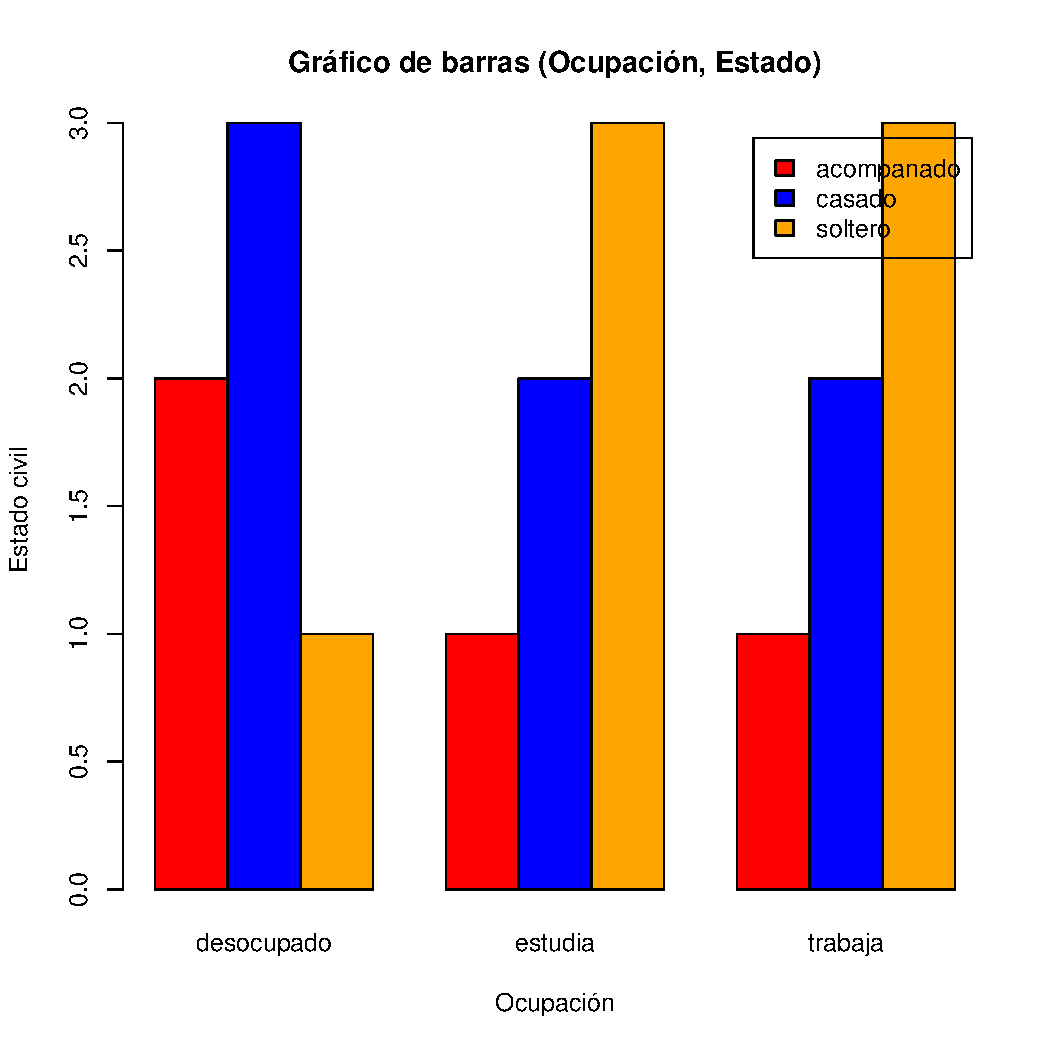
\includegraphics[width=\maxwidth]{figure/unnamed-chunk-19-1} 

\end{knitrout}

\begin{knitrout}
\definecolor{shadecolor}{rgb}{0.969, 0.969, 0.969}\color{fgcolor}\begin{kframe}
\begin{alltt}
\hlkwd{barplot}\hlstd{(}\hlkwd{table}\hlstd{(HojaCat),} \hlkwc{main}\hlstd{=}\hlstr{"Gráfico de barras (Ocupación, 
        Estado)"}\hlstd{,} \hlkwc{xlab}\hlstd{=}\hlstr{"Ocupación"}\hlstd{,} \hlkwc{ylab}\hlstd{=}\hlstr{"Estado civil"}\hlstd{,}
        \hlkwc{beside}\hlstd{=}\hlnum{TRUE}\hlstd{,}\hlkwc{col}\hlstd{=}\hlkwd{c}\hlstd{(}\hlstr{"red"}\hlstd{,} \hlstr{"blue"}\hlstd{,} \hlstr{"orange"}\hlstd{),}
        \hlkwc{legend.text}\hlstd{=}\hlkwd{c}\hlstd{(}\hlstr{"menor que 2"}\hlstd{,} \hlstr{"2-3"}\hlstd{,} \hlstr{"mayor que 3"}\hlstd{))}
\end{alltt}
\end{kframe}
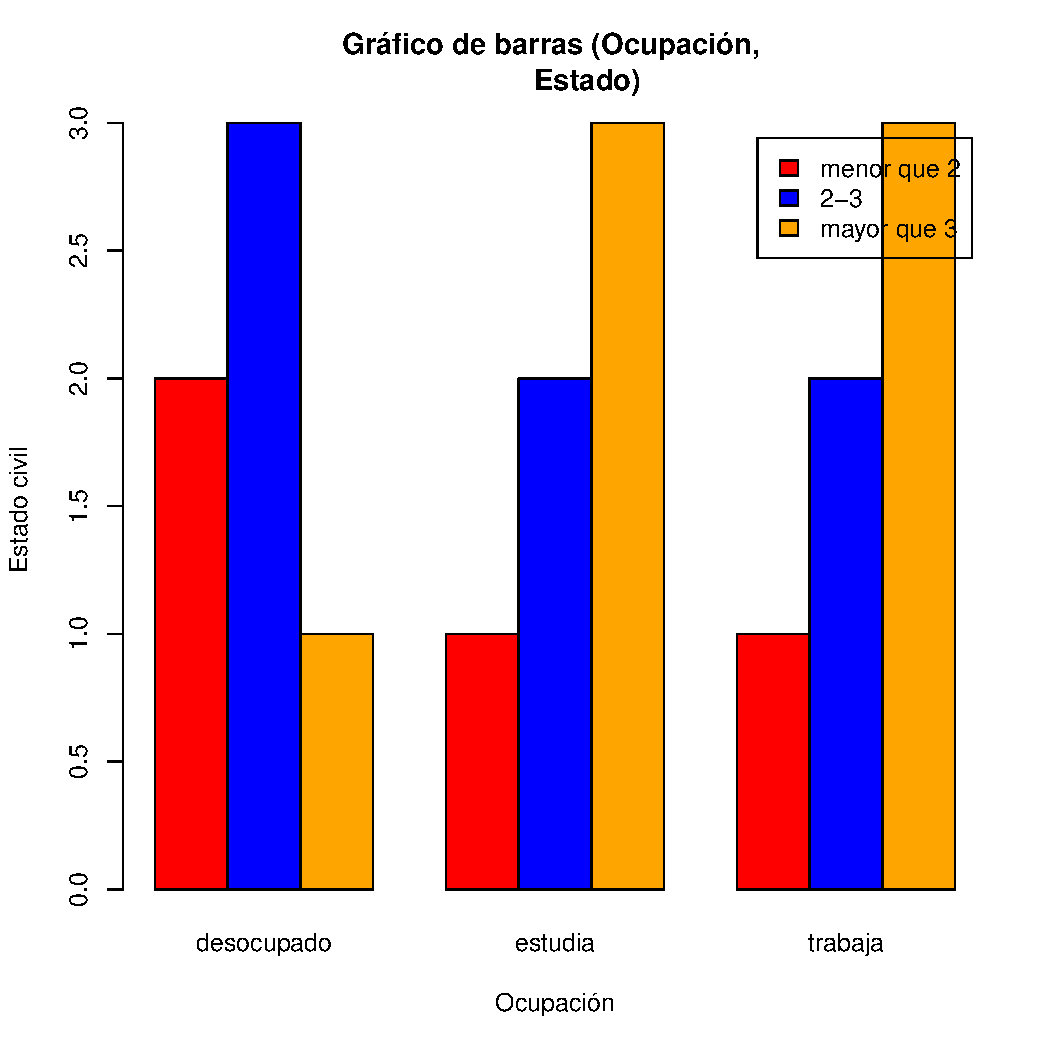
\includegraphics[width=\maxwidth]{figure/unnamed-chunk-20-1} 
\begin{kframe}\begin{alltt}
\hlcom{# Note que se puede definir a conveniencia la leyenda que se desea}
\hlcom{# incorporar en el grafico con la instruccion legend.text }
\end{alltt}
\end{kframe}
\end{knitrout}

\item Realizar la prueba o contraste Chi-cuadrado de independencia

\begin{knitrout}
\definecolor{shadecolor}{rgb}{0.969, 0.969, 0.969}\color{fgcolor}\begin{kframe}
\begin{alltt}
\hlstd{prueba} \hlkwb{<-} \hlkwd{chisq.test}\hlstd{(tablaCont); prueba}
\end{alltt}


{\ttfamily\noindent\color{warningcolor}{\#\# Warning in chisq.test(tablaCont): Chi-squared approximation may be incorrect}}\begin{verbatim}
## 
## 	Pearson's Chi-squared test
## 
## data:  tablaCont
## X-squared = 2, df = 4, p-value = 0.7
\end{verbatim}
\begin{alltt}
\hlcom{# Tenga en cuenta que las frecuencias esperadas deben ser todas mayores a 5 }
\end{alltt}
\end{kframe}
\end{knitrout}

\begin{knitrout}
\definecolor{shadecolor}{rgb}{0.969, 0.969, 0.969}\color{fgcolor}\begin{kframe}
\begin{alltt}
\hlcom{# Frecuencias absolutas esperadas para la prueba Chi-cuadrada }

\hlstd{prueba}\hlopt{$}\hlstd{expected} \hlcom{# fij = fi./No. column }
\end{alltt}
\begin{verbatim}
##             Ocupacion
## Estado.Civil desocupado estudia trabaja
##   acompanado       1.33    1.33    1.33
##   casado           2.33    2.33    2.33
##   soltero          2.33    2.33    2.33
\end{verbatim}
\end{kframe}
\end{knitrout}



















  
  
  
  
  
  
  
  
  
\end{enumerate}



\end{document}
